\subsection{\tkzname{范德瓦尔斯}曲线}

\bigskip
设 $v$ 为一定质量流体的体积，$p$ 为其压强。
$b$ 和 $k$ 为两个正实数。我们研究范德瓦尔斯提出的一个联系这些变量的公式。
\[
  p(v)= \frac{-3}{v^2} + \dfrac{3k}{v-b}
\]

定义在区间 $I=\tkzFnPrintInterval[oo]{b}{+\infty}$ 上。

\subsubsection{变化表}
\begin{center}
 \begin{tkzexample}[]
  \begin{tikzpicture}
  \tkzTab
  { $v$      /1,
    $g'(v)$  /1,
    $g(v)$   /3
  }
  { $b$ ,
    $3b$ ,
    $+\infty$
  }
  {0,$+$,$0$,$-$,t}
  {-/           $0$    /,
   +/$\dfrac{8}{27b}$  /,
   -/  $0$             /}
  \end{tikzpicture}
\end{tkzexample}
\end{center}

\newpage
\subsubsection{第一条曲线，\emph{b}=1}
 $1\leq v \leq 6$ 时的几条曲线

\medskip
\begin{center}
\begin{tkzexample}[]
\begin{tikzpicture}[xscale=2,yscale=2.5]
   \tkzFnInit[xmin=0,xmax=6,ymin=0,ymax=0.5,ystep=0.1]
   \tkzFnAxisX[ticks=false,label=$v$]
   \tkzFnAxisY[ticks=false,label=$g(v)$]
   \tkzFnGrid(0,0)(6,0.5)
   \tkzFnDraw[name=g,color=red,domain=1:6]{(2*(x-1)*(x-1))/(x*x*x)}
   \tkzFnTangent[color=blue,draw](g,3)
   \tkzFnText[draw,fill=brown!30](4,0.1){$g(v)=2\dfrac{(v-1)^2}{v^3}$}
\end{tikzpicture}
\end{tkzexample}
\end{center}

最大值在 $v=3$ 处取得：$g(3)=\dfrac{8}{27}\approx\tkzFnPrint[4]{g(3)}$。

\newpage
\subsubsection{第二条曲线，\emph{b}=1/3}

\medskip
\begin{center}
\begin{tkzexample}[]
\begin{tikzpicture}[scale=1.2]
  \tkzFnInit[xmin=0,xmax=2,xstep=0.2,ymin=0,ymax=1,ystep=0.1]
  \tkzFnAxes
  \tkzFnGrid(0,0)(2,1)
  \tkzFnDraw[name=g,color=red,domain=1/3:2]{(2*(x-1/3)^2)/x^3}
  \tkzFnTangent[draw,color=blue,kr=.5,kl=.5](g,1)
  \tkzFnText[draw,fill=brown!30](1.2,0.3)
             {$g(v)=2\dfrac{\left(v-\dfrac{1}{3}\right)^2}{v^3}$}
\end{tikzpicture}
\end{tkzexample}
\end{center}

\newpage
\subsubsection{第三条曲线，\emph{b}=32/27}

\medskip
\begin{center}
\begin{tkzexample}[]
\begin{tikzpicture}[scale=1.2]
    \tkzFnInit[xmin=0,xmax=10,ymin=0,ymax=.35,ystep=0.05]
    \tkzFnAxes
    \tkzFnGrid(0,0)(10,.35)
    \tkzFnDraw[name=g,color=red,domain=32/27:10]{(2*(x-32/27)^2)/x^3}
    \tkzFnTangent[draw,color=blue,kr=2,kl=2](g,{32/9})
    \tkzFnText[draw,fill=brown!30](5,0.3)
            {$g(v)=2\dfrac{\left(v-\dfrac{32}{27}\right)^2}{v^3}$}
\end{tikzpicture}
\end{tkzexample}
\end{center}

\newpage
\subsection{临界值}
\subsubsection{\tkzname{范德瓦尔斯}曲线}

\begin{tkzexample}[]
\begin{tikzpicture}[scale=4]
  \tkzFnInit[xmin=0,xmax=3,ymin=0,ymax=2]
  \tkzFnAxes
  \tkzFnGrid(0,0)(3,2)
  \tkzFnDraw[name=f,color=red,domain=1/3:3]{0.125*(3*x-1)+0.375*(3*x-1)/(x*x)}
  \tkzFnMarkPoints(f){2,3}
  \tkzFnTangent[draw,color=blue](f,1)
  \tkzFnDraw[name=g,color=green,domain=1/3:3]{0.125*(3*x-1)}
  \tkzFnMarkPoints[size=1pt,fill=orange](g){1/3,3}
  \tkzFnDefPointXY[draw,size=1pt,fill=orange](1,1){F}
  \tkzFnText[draw,fill=white,text=red](1,1.5)
  {$f(x)=\dfrac{1}{8}(3x-1)+\dfrac{3}{8}\left(\dfrac{3x-1}{x^2}\right)$}
  \tkzFnText[draw,fill=white,text=green](2,0.4){$g(x) = \dfrac{3x-1}{8}$}
\end{tikzpicture}
\end{tkzexample}

\newpage
\subsubsection{\tkzname{范德瓦尔斯}曲线（续）}

\tkzcname{foreach} 循环替代了四条定义；循环变量在表达式中使用。

\begin{tkzexample}[]
\begin{tikzpicture}[xscale=4,yscale=1.5]
  \tkzFnInit[xmin=0,xmax=3,ymin=-4,ymax=3]
  \tkzFnGrid(0,-4)(3,3)
  \tkzFnAxes
  \tkzFnVLine[color=red,dashed]{1/3}
  \foreach \a/\c in {0.5/red,0.84375/blue,1/orange,0.875/green}
    {\tkzFnDraw[color=\c,domain=0.35:3]{-3/(x*x)+8*\a/(3*x-1)}}
  \tkzFnText[draw,fill=white,text=Maroon](2,-2)
   {$f(x)=-\dfrac{3}{x^2}+\dfrac{8\alpha}{3x-1}$ \hspace{.5cm}
   其中 $\alpha \in
   \left\{\dfrac{1}{2}, \dfrac{27}{32}, \dfrac{7}{8}, 1\right\}$}
\end{tikzpicture}
\end{tkzexample}

\endinput
